\scanpage{9}

\textbf{ACADEMIE D'AIX-MARSEILLE}\\
\rule{3cm}{.4pt}\\
\textbf{INSPECTION ACADEMIQUE}\\
\textbf{DE VAUCLUSE}\\
\rule{1cm}{.4pt}
\mspage{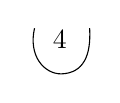
\begin{tikzpicture}[baseline=(n.base)]\node[inner sep=0pt] (n) at (0,0) {4};\draw (-.32,.15)..controls(-.4,-.2)and(-.2,-.43)..(.02,-.43)..controls(.3,-.42)and(.4,-.2)..(.38,.15);\end{tikzpicture}}
\[\begin{aligned}
p_{12}\delta_1(x)&=\sigma(x)\\
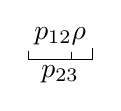
\begin{tikzpicture}[baseline=(t.base)]\node[inner sep=0pt] (t) {$p_{12}\rho$};\draw ([xshift=-2pt,yshift=-2pt]t.south west)--([xshift=-2pt,yshift=-5pt]t.south west)--([xshift=2pt,yshift=-5pt]t.south east)--([xshift=2pt,yshift=-1pt]t.south east);\draw ([xshift=4pt,yshift=-5pt]t.south)--++(0,2.5pt);\node[anchor=north,inner sep=0pt] at ([yshift=-7pt]t.south) {$p_{23}$};\end{tikzpicture}\delta_1(x)&=\delta_0p_0(x)\\
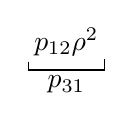
\begin{tikzpicture}[baseline=(t.base)]\node[inner sep=0pt] (t) {$p_{12}\rho^2$};\draw ([xshift=-2pt,yshift=-2pt]t.south west)--([xshift=-2pt,yshift=-5pt]t.south west)--([xshift=2pt,yshift=-5pt]t.south east)--([xshift=2pt,yshift=-1pt]t.south east);\node[anchor=north,inner sep=0pt] at ([yshift=-7pt]t.south) {$p_{31}$};\end{tikzpicture}\delta_1(x)&=x
\end{aligned}\]
\margin{NB $\delta_1(x)$ ne peut être fixe par $\rho$ (donc par $\unsure{\mathcal G_3|\mathfrak S_3}$) que si $x=\delta_0p_0(x)$ (condition néc. et suff.)}
\[\begin{tikzpicture}[baseline=(r.base)]
\node[inner sep=6pt] (r) {$\begin{gathered}\delta_0p_0(x)=1\\\sigma(x).x=1\\[.5em]p_{12}(z)p_{23}(z)p_{31}(z)=1\end{gathered}$};
\draw ([xshift=3pt,yshift=2pt]r.north west)--([xshift=-3pt,yshift=2pt]r.north east);
\draw ([yshift=-2pt]r.north west)--(r.south west)--(r.south east)--([yshift=-2pt]r.north east);
\end{tikzpicture}\]
\[\sigma(x)\begin{tikzpicture}[baseline=(t.base)]\node[inner sep=0pt] (t) {$\delta_0p_0(x)$};\draw ([xshift=-2pt,yshift=-2pt]t.south west)--([xshift=-2pt,yshift=-5pt]t.south west)--([xshift=2pt,yshift=-5pt]t.south east)--([xshift=2pt,yshift=-1pt]t.south east);\node[anchor=north,inner sep=0pt] at ([yshift=-7pt]t.south) {$\substack{\Vert\\1}$};\end{tikzpicture}x=1\]
pour $z\in E_2$ (une relation \deleted{\unsure{par|pour}} supplémentaire par orbite 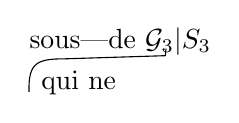
\begin{tikzpicture}[baseline=(w.base)]
\node[anchor=west,inner sep=0pt] (w) at (0,0) {qui ne};
\node[anchor=west,inner sep=0pt] at (-.15,.52) {\inserted{\unsure{sous|de} $\unsure{\mathcal G_3|\mathfrak S_3}$}};
\draw (-.15,-.12)..controls(-.16,.25)and(-.05,.3)..(.3,.3)--(1.58,.34)--(1.59,.43);
\end{tikzpicture} rencontre pas $\delta_1(E_1)$)
\diagram{\begin{tikzpicture}[x=1cm,y=1cm]
\node at (-.6,0) {$\delta_1$};
\node (top) at (1.8,0) {$F\times F\times F$};
\node at (1.8,1.45) {$\sigma_1$};
\draw (1.53,.63)..controls(1.15,.9)and(1.72,1.37)..(2.13,1.16)..controls(2.6,.96)and(2.24,.68)..(2.05,.61);
\draw (1.53,.63)--(1.58,.68);\draw (2.05,.61)--(2.01,.74);
\draw[line width=.7pt] (1.58,-.42)..controls(1.52,-.3)and(1.56,-.95)..(1.58,-1.12);
\draw[line width=.7pt] (1.46,-1.01)--(1.58,-1.12)--(1.7,-1.02);
\node at (1.08,-.7) {$p_{12}$};
\draw[line width=.7pt] (2.14,-.37)..controls(2.03,-.25)and(2.08,-.93)..(2.13,-1.1);
\draw (2.13,-1.1)--(2.12,-.31)--(2.29,-.44);
\draw[line width=.7pt] (2,-.98)--(2.13,-1.1)--(2.28,-.99);
\node at (2.7,-.7) {$p_{13}$};
\draw (top.east)..controls(4.1,.24)and(6,.38)..(8.2,.4);
\draw (4.13,-.03)..controls(5.65,.37)and(6.9,.17)..(7.53,.18)--(7.48,.27);
\node at (6.5,-.9) {$\alpha\in E_1$};
\node at (-.2,-1.7) {$F_\alpha$};\node at (.7,-1.7) {$\subset$};
\node at (1.8,-1.7) {$F\times F$};
\draw (1.83,-2.08)--(1.86,-2.95);\draw (1.72,-2.82)--(1.86,-2.95)--(2,-2.83);
\node at (2.36,-2.45) {$\mathrm{pr}_0$};\node at (1.86,-3.25) {$F$};
\end{tikzpicture}}
\[(x,y)\mapsto y\]
\[(x,y)\times_{\unsure{y|x}}\unsure{x'|x^+},y')\sim(x,\deleted{y},y')\]
\[\Pi_0(F_\alpha\times_F F_\alpha)=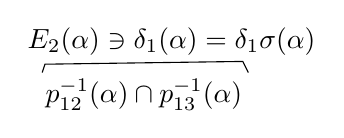
\begin{tikzpicture}[baseline=(t.base)]
\node[inner sep=0pt] (t) {$p_{12}^{-1}(\alpha)\cap p_{13}^{-1}(\alpha)$};
\draw ([xshift=-1pt,yshift=2pt]t.north west)--([xshift=0pt,yshift=5pt]t.north west)--([xshift=0pt,yshift=6pt]t.north east)--([xshift=2pt,yshift=2pt]t.north east);
\node[anchor=south,inner sep=0pt] at ([xshift=10pt,yshift=8pt]t.north) {$E_2(\alpha)\ni\delta_1(\alpha)=\delta_1\sigma(\alpha)$};
\end{tikzpicture}\qquad\text{stable par }\sigma_1\]
\margin{Le petit coq aux champs\\\deleted{\unsure{tél}}\\$\boxed{32\ 41\ 04\ 19}$}
\margin{$y,x,y$}
Prenons $\alpha\ne\delta_1$, alors $\delta_2\notin p_{12}^{-1}(\alpha)$

les p\textsuperscript{ts} fixes par $\sigma_1$ sont dans image $\delta_1(E_1)$, mais $p_{12}(\delta_1(x))=p_{13}(\delta_1(x))=\sigma x$, donc \deleted{\unsure{il faut}}
\deleted{\unsure{faut} $\sigma x={}$} $\delta_1(x)\in E_2(\alpha)\Longleftrightarrow\overset{!}{\sigma}x=\alpha$ i.e. $x=\uline{\sigma\alpha}$

et $\uline{\delta_1\sigma}(\alpha)$ joue le rôle de $\delta_2=\delta_1(\alpha)$
\margin{8}
